%===================================== CHAP 4 =================================

\chapter{Implementation}\label{chap:implementation}

This chapter thoroughly describes the implementation process and the implementation itself, for both the visualization tool and the networks implemented for the case study. For clarity, all code examples in this chapter have omitted comments and code irrelevant to the example.

\section{Visualization Tool}

In this section we will present the implementation details of the visualization tool created as part of the thesis. We start with a summary of the related results from the Specialization Project, before explaining the system development methodology used in the implementation process. Then, we present the two quality attributes that have been focal points throughout the design and implementation phase, and state our choices regarding the technology used. Finally, we showcase the implementation details for the main parts of the visualization tool. \\

\noindent Note that this section does not explain how to install or use the visualization tool. This is described in \autoref{app:installation-setup} and \autoref{app:user-manual}, respectively.

\subsection{Prototype}

This section presents the results from the Specialization Project in terms of the previously implemented prototype of the visualization tool, as well as some pointers on the planned improvements and extensions to be included for the thesis.

\subsubsection{Description}

\noindent The prototype provides all the basic user functionality for creating a user, and logging in and out, including validation of the user name and password. Once created, a user can upload Python scripts from their computer to the server, and tag them with various labels to make them easier to search for. The search bar is located on a page showing all uploaded scripts. \\

\noindent By selecting a specific script, the user can view its code, and add and delete tags associated with it. The user can also run the script, or delete it. A separate menu tab for the visualizations grants the user access to visualizations of the data produced during script execution. The visualizations available are the training progress and the layer activations, both presented on a single page. The training progress includes two separate plots showing the training accuracy and loss over the batches, while the layer activations are shown for each single layer of the script-defined network.

\subsubsection{Regarding Planned Improvements and Extensions}

The Specialization Project provided a list of major and minor extensions that would be useful to implement in an improved version of the visualization tool. Upon beginning the thesis work, the main focus of the thesis was shifted from the face recognition study to the visualization tool. Instead of the tool being created for the purpose of aiding our case study effort, the goal is now to release the code as open-source software for the benefit of other researchers. As a result, we have focused on properly implementing and testing the user functionality and visualization techniques for general networks. The tool supports fully sequential networks, but because of resource limitations, support for non-sequential models has not been added. There was also a shift in the use of the tool, namely that instead of a web application running on a server, it would be a desktop application that the user runs in a web browser. The user system is kept because it still has value in certain scenarios. For instance, if a lab provides a powerful computer used to train \acrshortpl{ann} that several people have access to. \\

\noindent The move to a desktop application affected the relevance of certain planned extensions, and we have therefore decided to discard some of them. However, the two most important extensions were added: allowing a user to download a network, and implementing the saliency maps, deconvolutional network and deep visualization techniques. In addition, we have added more functionality, like stopping the execution of a script, using user uploaded images in visualizations, and viewing the console output produced by the script. The presentation of the visualizations have also been improved, making them more interactive and readable.

\subsection{System Development Methodology}

The development of the visualization tool has been carried out by a team of two, with no specific set of roles involved. On account of the small team size, a dedicated project manager was not deemed necessary. Both team members were involved in the design of the architecture and interface, as well as system implementation and testing. An efficient workflow was maintained by dividing the programming work into two main areas of responsibility:
\begin{enumerate}
    \item Implementing visualization techniques and creating networks to produce example data.
    \item Implementing visualization data processing and presenting the result to user interface.
\end{enumerate}

\noindent The development process itself did not follow any strict guidelines, but included several elements from Agile methods\footnote{https://www.agilealliance.org/}. It has been an iterative and incremental process, starting with the existing prototype of the system that only implemented two of the visualization techniques. Based on our own testing, as well as feedback from our supervisors, functionality was added and adjustments were made in order to obtain a new and improved prototype. This process was repeated until we reached a satisfactory system according to the initial requirements. An example of the iterative part of the process is the replacement of the old visualization library in favor of a new one that was better suited for visualization interactivity and streaming of real-time data. An example of the incremental part of the process is the shift to user-uploaded images for usage in certain visualization techniques, which was added after supervisor feedback. Other concepts from Agile development that were applied are code review, pair programming, and the use of a backlog to get an overview of the requirements.

\subsection{Focus Quality Attributes}

In addition to functional requirements, we wanted to incorporate some non-functional requirements as well. To that end, we have selected two quality attributes that we consider to be of high importance. Quality attributes are overall factors that represents areas of concern which impact the application as a whole. In our case, we have determined that the most important factors are modifiability and usability.

\subsubsection{Modifiability}

An important aspect of the visualization tool's system design was to ensure that certain parts could be easily replaced. For instance, a user should be able to alter the system to employ a different deep learning library than Keras without much difficulty. This requires thorough consideration when designing the architecture, and typically calls for a module-based architecture with loosely coupled modules, meaning that each module should interact with as few of the other modules as possible.

\subsubsection{Usability}

Not only should the interface be simple and easy to navigate for the user, but the actual installation and setup of the visualization tool should be straightforward. In addition, the tool's requirements for the user scripts should be easy to fulfill. A comprehensive user manual and documentation of the \acrshort{api} is the key to obtaining this kind of usability. Preferably, we would want any \acrshort{ann} to run in our program without issues, but the extensive variety of network architectures makes it incredibly difficult to acquire such generalization. Consequently, we prioritized supporting the most common architectures.

\subsection{Technology Decisions}

This section presents the technology used in our implementation, as well as justification of why they were selected and identification of any potential drawbacks.

\subsubsection{Flask}

Flask\footnote{http://flask.pocoo.org/} is a web framework for Python, used to build simple web applications. It is a micro-framework, meaning that it has a minimal amount of dependencies on external libraries. It provides only the basic tools needed to create a web application, and is therefore very lightweight. However, there exist many plugins that can be added for an increased range of functionality. Since the focus of our application is not the web page itself, but rather its capabilities in terms of visualization techniques, Flask was the perfect choice. Together with a selection of plugins, it allowed us to quickly set up an application and implement a basic user system and upload functionality.

\subsubsection{SQLite}

SQLite\footnote{https://www.sqlite.org/} is a simple and lightweight relational SQL database engine. In contrast to many other databases, it is embedded into the application. It is often used to provide local data storage for desktop applications. An embedded database improves application performance, reduces cost and complexity, and improves reliability. The visualization tool does not require any advanced database functionality, nor does it store large amounts of data or utilize many database connections simultaneously. The lightweight SQLite therefore represents a suitable choice. Additionally, it is uncomplicated to set up, and could be easily replaced with a more advanced database system at a later time, if needed.

\subsubsection{Keras}

Keras\footnote{https://keras.io/} is a high-level neural networks library that can run on top of either TensorFlow\footnote{https://www.tensorflow.org/} or Theano\footnote{http://deeplearning.net/software/theano/}. Its purpose is to facilitate quick and easy creation of networks and, by extension, rapid experimentation. Keras offers a wide range of network functionality, enveloped in a straightforward and well documented \acrshort{api}. It also has a strong modifiability basis, making it easy for users to create functional extensions using custom modules. The library contains several callbacks, which are sets of functions to be applied at given stages of the \acrshort{ann} training procedure. It also allows for creating custom callbacks, which is advantageous when we want to apply various visualization techniques at certain stages of training. Consequently, we chose to develop our visualization tool with support for Keras including both the TensorFlow and Theano backend. The use of Keras is strictly limited to the callbacks, to ease a potential substitution of the deep learning library.

\subsubsection{Bokeh}

Bokeh\footnote{http://bokeh.pydata.org} is a Python-based interactive visualization library for modern web browsers. It can be embedded into a Flask application without difficulty, as described later in the chapter. The library is easy to use, and provides the flexibility of adding interactions and advanced customization without much effort. Another benefit is that it allows for streaming large data sets and plot them live, a highly useful feature for our application. However, Bokeh is still in an early state of development, which makes it more susceptible to bugs, and will in some cases limit its functionality.

\subsection{Overview of the Architecture}

As seen in \autoref{fig:overall-architecture}, the system can be divided into five separate modules: the user storage, Bokeh, Flask, Keras and the database. The Flask module represents the core of the application. It defines the routes (URLs), models and forms of the web pages, tying the functionality together with HTML templates, CSS and JavaScript into a simple web interface. The user storage contains all the scripts and images that are uploaded through the Flask application, as well as the visualization data produced during network training. The database stores the metadata concerning the uploaded scripts, such as file owner, upload timestamp, and the file path. The Keras module includes the custom callbacks created for the visualization techniques. These write data to the files saved in the user storage. To include a specific visualization technique, a user simply includes the corresponding callback in his or her script. It is the Flask application that implements the functionality for executing these scripts. Finally, the Bokeh module uses the data located in the user storage to create interactive visualizations, and the Flask application handles how these are displayed in the web interface. \\

\noindent A package diagram in \autoref{fig:package-diagram} shows a more low-level view of the architecture. There are three packages: \texttt{custom\_keras}, \texttt{custom\_bokeh} and \texttt{visualizer}, which correspond to the Keras, Bokeh and Flask modules, respectively. In this case, a package corresponds to a folder inside of the main project folder. The folders and the files they contain are displayed, as well as the dependencies between them. The packages will be explained in further detail in the following sections.

\begin{figure}[h!]
    \centering
        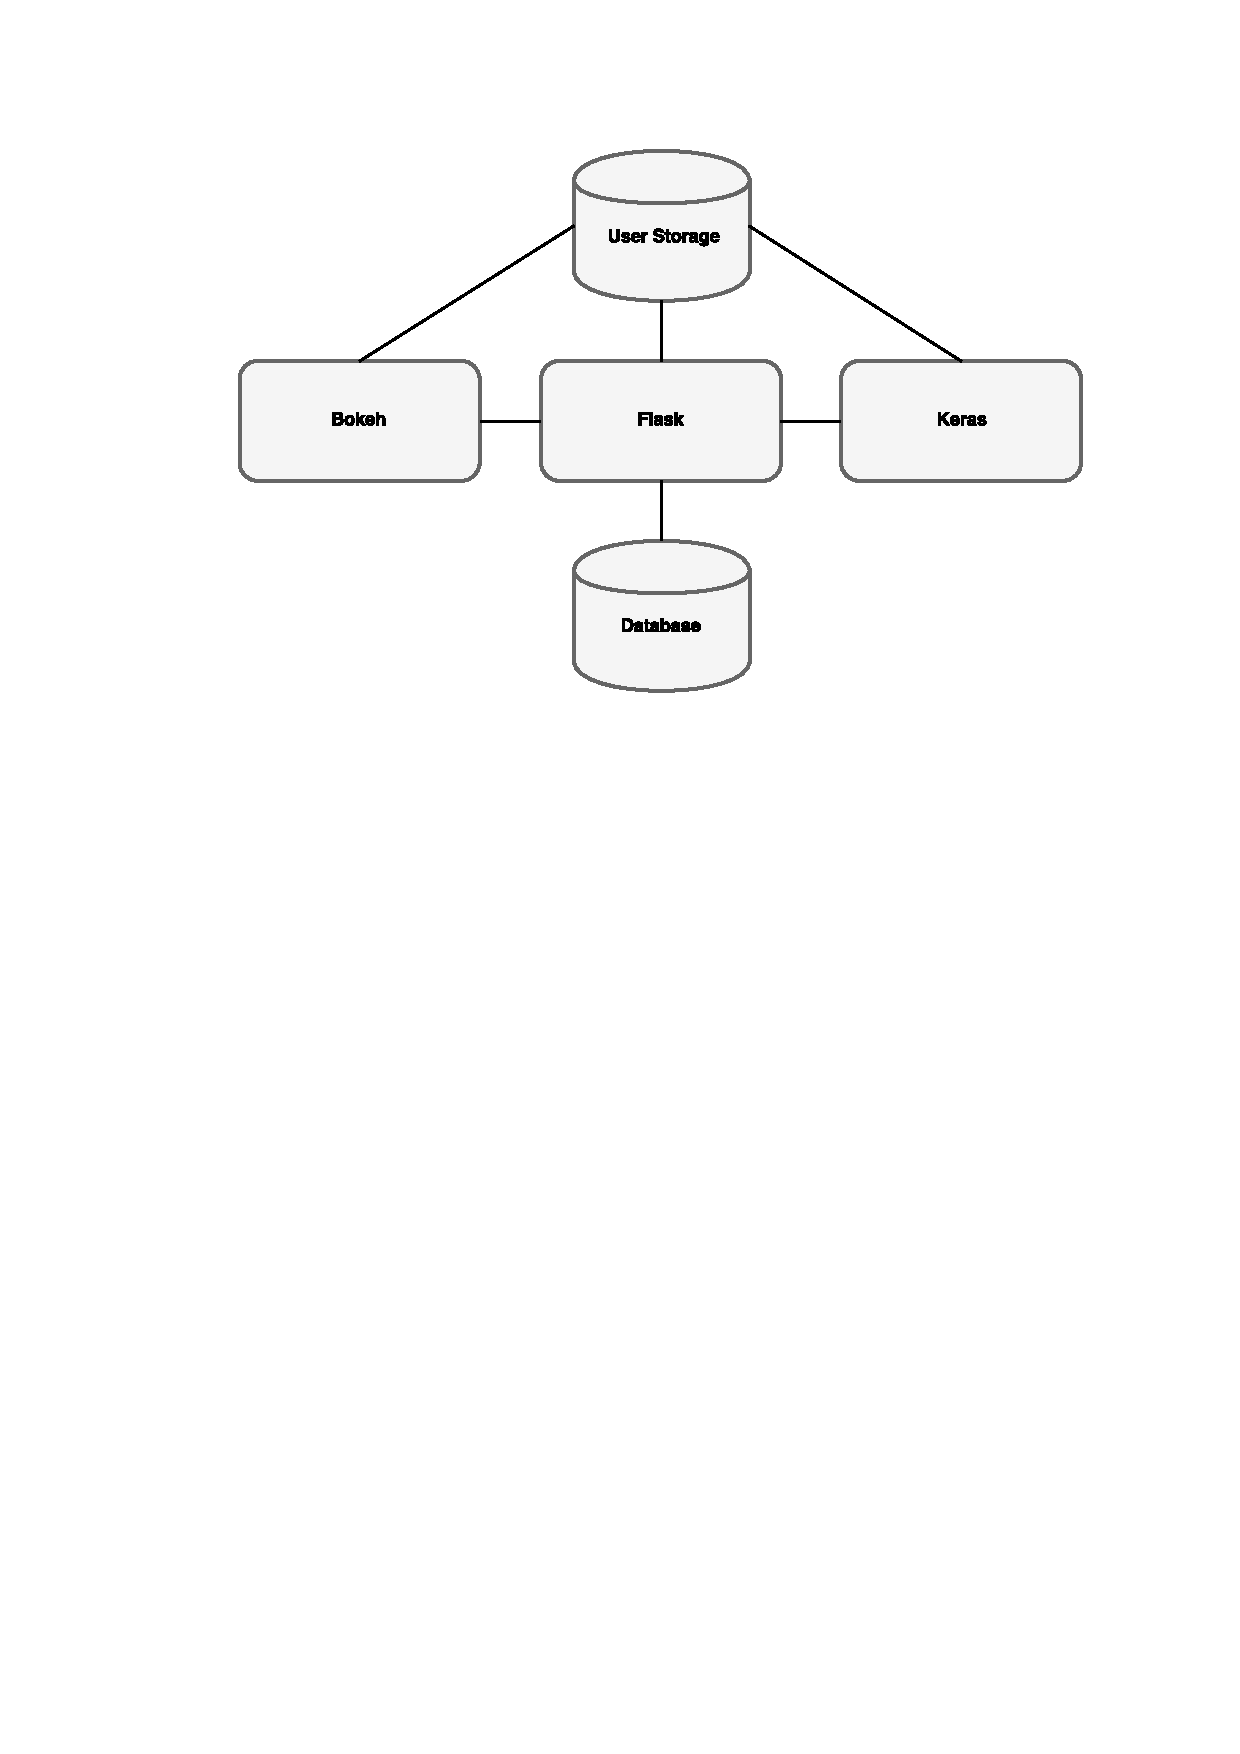
\includegraphics[width=0.8\textwidth]{fig/overall-architecture.pdf}
        \caption{Overall Architecture of the System}
        \label{fig:overall-architecture}
\end{figure}

\begin{figure}[h!]
    \centering
        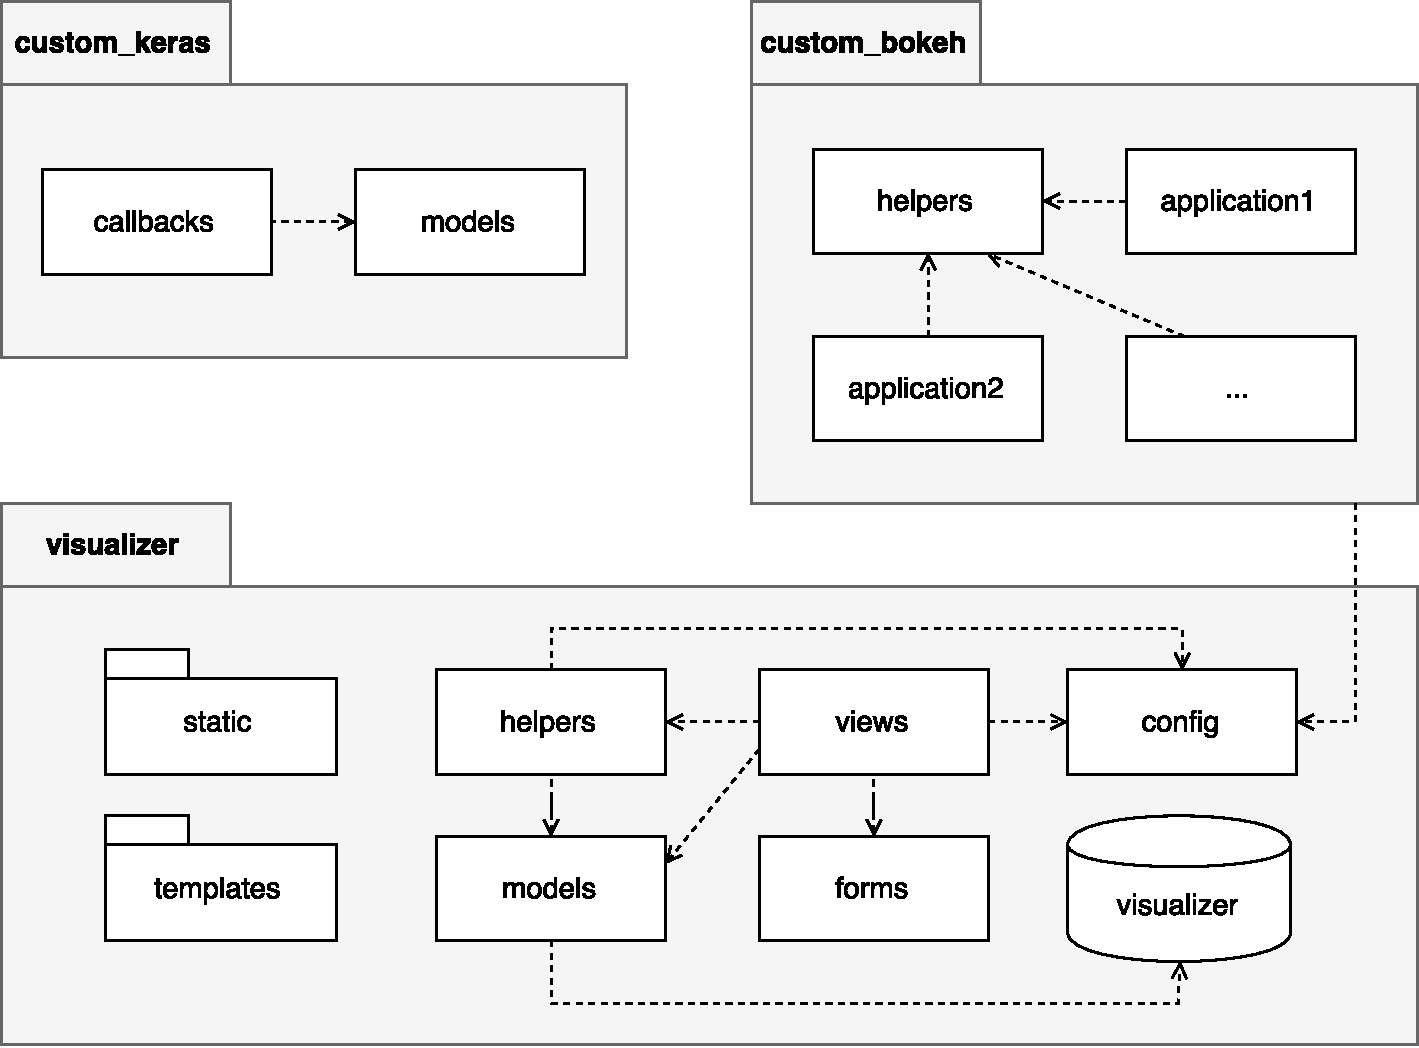
\includegraphics[width=\textwidth]{fig/package-diagram.pdf}
        \caption{Package Diagram}
        \label{fig:package-diagram}
\end{figure}

\subsection{The Flask Application}

\autoref{fig:file-structure} shows an overview of the structure of the files that are included in the Flask application. The \texttt{static} folder serves all the CSS and JavaScript files, while the \texttt{templates} folder contains Jinja2 \footnote{http://jinja.pocoo.org/} templates that Flask can render to generate the HTML. The \texttt{\justify\_\_init\_\_.py} file contains the instantiation of the Flask application, as well as partial setup for the database and login system. The \texttt{config.py} file configures certain application parameters, such as setting the system commands necessary for running Python scripts. The database, \texttt{visualizer.db}, and the \texttt{user\_storage} folder are also seen in the file structure. These will be further explained in \autoref{sec:database} and \autoref{sec:user-storage}, respectively.\\

\begin{figure}[h!]
\begin{verbatim}
/visualizer
    /static
        /css
        /fonts
        /js
    /templates
        /create_user.html
        /home.html
        /layout.html
        /...
    /user_storage
        /...
    /__init__.py
    /config.py
    /forms.py
    /utils.py
    /models.py
    /requirements.txt
    /views.py
    /visualizer.db
\end{verbatim}
\caption{Flask project file structure}
\label{fig:file-structure}
\end{figure}

\noindent There are three main files implementing the functionality of the Flask application: \texttt{forms\-.py}, \texttt{models.py} and \texttt{views.py}. They define all the forms, models and views, respectively, of the web interface. A form is used to collect user input, for instance when registering a new user, or uploading a script. Models are used to create database objects, which are explained in the next section. Lastly, a view defines a URL endpoint, or a route, as well as what HTTP requests it answers to, and determines what the system should do when a user navigates to that URL. There also exists a \texttt{utils.py} file that contains various utility methods. \\

\noindent An example of a view from \texttt{views.py} is shown in  \autoref{code:create-user}. Line 1 defines the route of the view and the HTTP requests to answer to, which is GET and POST. GET is used for returning the user register page, while POST is used when the register button is actually clicked. The code illustrates the use of a form in line 3, in this case for creating a new user, which will contain the chosen username and password of the new user. Line 5 checks if all the form fields are valid when a user has submitted a POST request, while the next line alerts the user and halts the process if the username is already taken. If not, line 9 creates a User database entry consisting of the username and password and adds it to the database. Note that the password is salted and hashed upon entry creation, for security reasons. Line 13 redirects the user to another view, namely the login view. If the user has not submitted a form, or the submission was unsuccessful, line 15 ensures that the correct template for the user registration page is rendered. \\

\begin{listing}[h!]
\begin{minted}
[
frame=lines,
framesep=2mm,
baselinestretch=1.2,
fontsize=\footnotesize,
linenos
]
{python}
@app.route('/create_user', methods=['GET', 'POST'])
def create_user():
  form = CreateUserForm()
	
  if form.validate_on_submit():
    if not unique_username(form.username.data):
      flash('Username is already taken', 'danger')
    else:
      db.session.add(User(form.username.data, form.password.data))
      db.session.commit()
			
      flash('User successfully created', 'success')
      return redirect(url_for('login'))
		
  return render_template('create_user.html', form=form)
\end{minted}
\caption{View for creating a user}
\label{code:create-user}
\end{listing}

\subsection{Database} \label{sec:database}

As mentioned earlier, the database is quite simple, and does not store a large amount of information. Its purpose is to handle the user system and store useful meta data about the uploaded scripts. It consists of three models, with attributes and connections as seen in \autoref{fig:database-diagram}. The \texttt{User} model contains necessary information of a user. The \texttt{FileMeta} model contains the meta data of the scripts, as well as a connection to its owner. There is also a separate \texttt{Tag} model, that can be associated to zero, one, or several scripts.

\begin{figure}[h!]
    \centering
        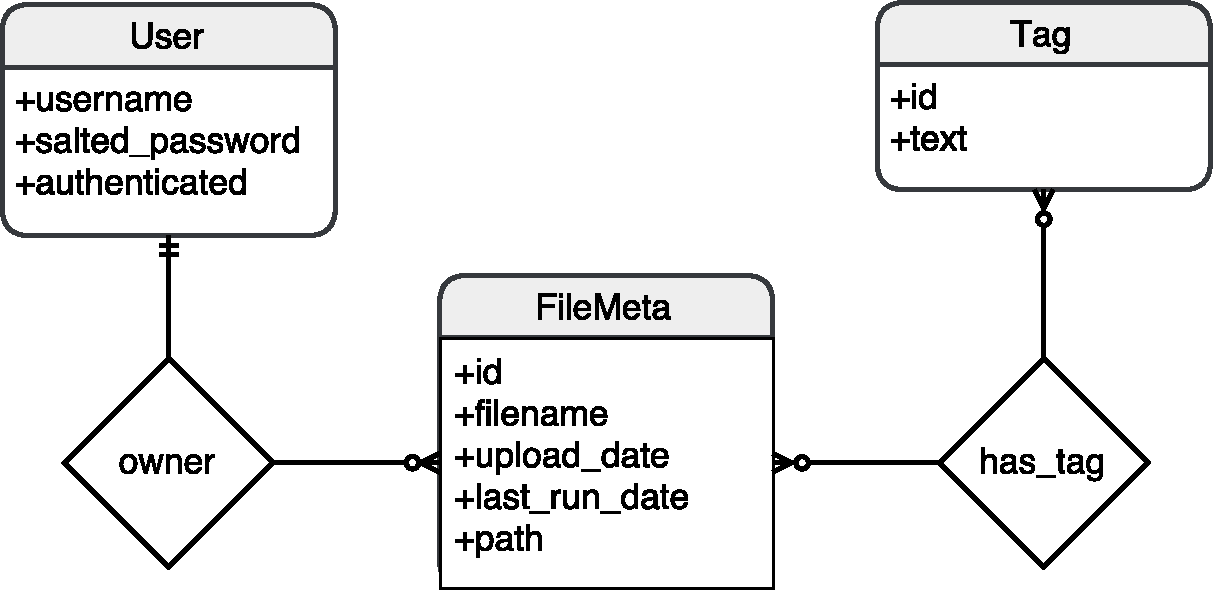
\includegraphics[width=0.7\textwidth]{fig/database-diagram.pdf}
        \caption{ER-diagram of the database}
        \label{fig:database-diagram}
\end{figure}

\subsection{User Storage} \label{sec:user-storage}

The user storage is where the scripts are uploaded to, and where the visualization data is stored. The structure of the user storage can be seen in \autoref{fig:user-storage}. The top level holds the different users of the system. The second level contains the various scripts that a user has uploaded. At the next level, the script file itself is stored, as well as a text file containing the console output of the script. There is a folder called \texttt{images} that contains the image that the user has uploaded to be used in the visualizations. The \texttt{networks} folder contains the most currently saved network created by the script. The folder called \texttt{results} stores all the data produced by the various callbacks. The files are all given descriptive names so that it is self-evident which file corresponds to which visualization technique. The format of the visualization files are presented in \autoref{app:visualization-files}.

\begin{figure}[h!]
\begin{verbatim}
/user-storage
    /<user1>
        /<script1>
            /images
                /<image>
            /networks
                /<network>
            /results
                /deconvolutional_network.pickle
                /deep_visualization.pickle
                /layer_activations.pickle
                /saliency_maps.pickle
                /training_progress.txt
                /training_progress_val.txt
            output.txt
            <script1>
        /<script2>
            /...
    /<user2>
        /...
\end{verbatim}
\caption{User storage structure}
\label{fig:user-storage}
\end{figure}

\subsection{Running a Python Script}

The visualization tool allows a user to both start and stop the uploaded Python scripts. Functionality for running a script is implemented as a utility function, and is done by executing \texttt{python [file\_path]} in a new subprocess, as seen in \autoref{code:run-script}. The actual Python command is determined by a configuration variable, since it is dependant on the user's Python installations (some systems use \texttt{python3} for Python 3.x and simply \texttt{python} for Python 2.x). The \texttt{stdout} argument specifies the standard output file handle, which is in this case a text file that will be displayed in the web interface, so that the user is given easy access to the console output of the script. Note that even though \autoref{fig:overall-architecture} shows a connection between Keras and Flask, the real connection is really between Python and Flask. A user could easily upload a Python script that uses the scikit-learn library\footnote{http://scikit-learn.org/stable/} or pure TensorFlow, and running such a script would not cause any issues. However, if someone wanted to adapt the visualization tool to a whole different programming language, this section of the code would need to be replaced.

\begin{listing}[h!]
\begin{minted}
[
frame=lines,
framesep=2mm,
baselinestretch=1.2,
fontsize=\footnotesize,
]
{python}
with open(get_output_file(get_current_user(), basename(file_path)), 'w') as f:
  p = subprocess.Popen([PYTHON, file_path], stdout=f)
\end{minted}
\caption{Running a Python script using subprocess}
\label{code:run-script}
\end{listing}

\subsection{Custom Keras Callbacks}

The custom callbacks are the only part of the visualization tool that are specific to Keras. As mentioned, a callback is a set of functions to be applied at given stages of the \acrshort{ann} training procedure. Keras provides several predefined callbacks, but also includes the possibility of creating custom variations. We have taken advantage of this functionality, and have created a callback for each visualization technique, as well as for other useful functionality. An overview of the custom callbacks, and how to adapt them to your script, is thoroughly explained in \autoref{app:callbacks-api}. In addition, we will also showcase certain parts of their implementation in this section. The implementation of the visualization functionality in the callbacks follows the processes explained in \autoref{sec:visualization-theory} quite strictly. Consequently, these parts will not be examined any further here. We will, however, explain the implementation details of the deconvolutional network that are not covered by the background theory. 

\subsubsection{CustomCallbacks - A Wrapper Class for the Custom Callbacks}

Every custom callback requires the system path to the folder containing the script they are to be used in. In addition, a subset of the callbacks share similar, optional arguments. To simplify the user's process of adding callbacks to their code, we have created a wrapper class that takes all the common arguments on its instantiation. The wrapper class also provides methods for registering each callback with their associated arguments, excluding the shared ones, and a method for getting the list of registered callbacks. A user can apply their selected callbacks by passing this list to the \texttt{callbacks} argument of the \texttt{.fit()} method of a Keras model.\\

\noindent An excerpt of the implementation of the wrapper class is shown in \autoref{code:wrapper-class}. There you can see the initialization of an instance of the class, which instantiates the necessary and optional variables in lines 3-10. The argument named \texttt{file\_folder} is the path to the folder of the script the callbacks are applied to, denoted as \texttt{<script1>} and \texttt{<script2>} in \autoref{fig:user-storage}. This is needed to know where the callbacks should store their produced data. The arguments \texttt{custom\_preprocess} and \texttt{custom\_postprocess} are functions that can be defined by the user to pre- and post-process images to be used in visualization. The argument named \texttt{base\_interval} is the batch interval that each callback is applied at, unless overridden at callback registering. The callbacks vary in their computational complexity, and some of them take significantly longer to execute than others. These have their own interval argument that supersedes the base interval. \\

\noindent The excerpt also shows two of the register methods of the wrapper. The first one, named \texttt{register\_training\_progress} , seen in line 15, simply creates a new instance of the \texttt{TrainingProgress} callback, using the previously defined file folder as a parameter, and adds it to the callback list. The second method, named \texttt{register\_saliency\_\-maps}, in line 18, does the exact same thing, except that it also uses the aforementioned interval argument. If the user does not specify an alternate interval upon registering, the interval of the callback is set to the base interval. The pre- and postprocess functions, if specified, are also passed to the callback. The method in line 12 returns the list of all added callbacks.

\begin{listing}[h!]
\begin{minted}
[
frame=lines,
framesep=2mm,
baselinestretch=1.2,
fontsize=\footnotesize,
linenos
]
{python}
class CustomCallbacks:

  def __init__(self, file_folder, custom_preprocess=None, 
               custom_postprocess=None, base_interval=10):
		
    self.file_folder = file_folder
    self.custom_preprocess = custom_preprocess
    self.custom_postprocess = custom_postprocess
    self.base_interval = base_interval
    self.callback_list = []
		
  def get_list(self):
    return self.callback_list
		
  def register_training_progress(self):
    self.callback_list.append(TrainingProgress(self.file_folder))
		
  def register_saliency_maps(self, interval=None):
    if interval is None:
      interval = self.base_interval
    self.callback_list.append(SaliencyMaps(self.file_folder, 
                                           self.custom_preprocess, 
                                           self.custom_postprocess, 
                                           interval))
\end{minted}
\caption{Wrapper class for custom callbacks}
\label{code:wrapper-class}
\end{listing}

\subsubsection{Example Implementation of a Callback}

The implementation of the \texttt{LayerActivations} callback can be seen in \autoref{code:callback}. Specific functionality is omitted, as the purpose is to showcase the general approach. As all the custom callbacks, it is an extension of the base abstract class \texttt{keras.callbacks.Call\-back} as seen in line 1. The initialization takes all necessary and optional arguments, and set the attributes accordingly. The folder to save the data is obtained by adding 'results' to the \texttt{file\_folder} argument. The counter variable is set to one less than the interval so that an initial visualization will be produced. Line 13 starts the process of getting the visualization image and converting it to the correct format. In line 19, the preprocess function is applied if the user has specified one. \\

\noindent The \texttt{keras.callbacks.Callback} abstract base class defines various methods that are called at specified events, such as \texttt{on\_batch\_end} and \texttt{on\_train\_begin}, that are used in this example. In other custom callbacks, \texttt{on\_epoch\_end} is also used. In line 24, at the beginning of the training process, we call \texttt{on\_batch\_end} with the batch number 0 to produce the initial visualization. The counter value is increased in line 28, and line 31 checks whether it is time to perform the computation of the visualization data. The specific functionality varies from the different visualization techniques. Finally, line 35 creates the correct file for storing the data, in this case in a pickle file, and the counter is reset in line 39. Note that some of the callbacks also make use of a postprocess function, which would be applied to the visualization output before saving it. 

\begin{listing}[p]
\begin{minted}
[
frame=lines,
framesep=2mm,
baselinestretch=1.2,
fontsize=\footnotesize,
linenos
]
{python}
class LayerActivations(Callback):

  def __init__(self, file_folder, exclude_layers=EXCLUDE_LAYERS, 
               custom_preprocess=None, interval=10):

    super(LayerActivations, self).__init__()
    self.results_folder = join(file_folder, 'results')
    self.interval = interval
    self.counter = interval - 1

    self.exclude_layers = exclude_layers
		
    images_folder = join(file_folder, 'images')
    img_name = listdir(images_folder)[-1]
    img = Image.open(join(images_folder, img_name))
    self.img_array = img_to_array(img)

    if custom_preprocess is not None:
      self.img_array = custom_preprocess(self.img_array)
		
    self.img_array = np.expand_dims(self.img_array, 0)

  def on_train_begin(self, logs=None):
    self.on_batch_end(0)

  def on_batch_end(self, batch, logs={}):

    self.counter += 1
    layer_tuples = []

    if self.counter == self.interval:

      # specific functionality, removed to simplify example

      with open(join(self.results_folder, 
                     'layer_activations.pickle'), 'wb') as f:
        pickle.dump(layer_tuples, f)

      self.counter = 0
\end{minted}
\caption{Example implementation of a callback}
\label{code:callback}
\end{listing}

\subsubsection{Deconvolutional Network Implementation Details}

Using the deconvolutional network visualization technique requires a deconvolutional network which can reverse the mapping from input to features that the convolutional part of the original network performs. In the implemented callback for this technique, the deconvolutional network can be automatically generated for simple models. The generation process is restricted to building a model corresponding to a continuously convolutional part that represents the first component of the original network. For example, if a fully connected layer separates two convolutional parts, only the first part is considered when constructing the deconvolutional network. The generation is also limited to convolutional parts which contain layers using convolution or max pooling. Before the process can start, the convolutional part is identified by examining the original network. This part is explored from top to bottom, while the deconvolutional network is being built from the bottom up. For every convolutional layer in the original, the appropriate deconvolutional substitute is added. Concurrently, a map concerning corresponding original and deconvolutional layers is being created. If a deconvolutional model cannot be created, the user must build the model and pass it to the callback. \\

\noindent To approximately reverse the effects of max pooling layers, the auto-generated deconvolutional networks use a custom Keras layer we have created called MaxUnpooling2D. These layers are used instead of the switch variables described in \autoref{sec:unpool-theory}, as this would require interfering with the uploaded networks, which could have unforeseen consequences. MaxUnpooling2D layers are image specific, which in turn make the deconvolutional models using them image specific. They compute the pooling regions used in the original max pooling based on the region size, strides, padding, as well as the shape of the input and output. These regions are computed differently for Theano and TensorFlow, depending on the aforementioned values. Then, for each region, the layer identifies which position the original max value was selected from by examining the original input and output. Subsequently, a zero matrix the size of the original input is created, and the max positions are filled with their corresponding values in the MaxUnpooling2D input. Thus, the functionality of the switch variables have been reproduced, without altering the original network.  \\

\noindent When visualizing via the web interface, the deconvolutional network will either identify and visualize the feature maps that maximally activate on the user uploaded image, or visualize the feature maps directly specified by the user. Which of these options are chosen are based on the arguments passed when instantiating the callback. The arguments are explained further in \autoref{app:callbacks-api}. The callback only allows visualization of feature maps from a single layer, but there is no limit on the amount of feature maps from the chosen layer. In addition to these alternatives, we have also implemented functionality that produces visualizations for a set of images that maximally activate certain feature maps. The feature maps can either be specified directly or a given amount can be randomly sampled. A large set of images will then be examined for each of these feature maps, computing the activation for each one. A predefined amount of images are selected for each chosen feature map, and their deconvolutional visualizations are produced. The max activation images represent samples that specifically contain the feature that the map's corresponding filter is looking for, and the visualizations of these images will highlight that feature. The image set from which the max activation images are sampled is based on the 2011 \acrshort{ilsvrc} object classification image set \cite{imagenet}. This functionality is not available in the tool, however, as it was found to be prohibitively slow in its current state. Although it was implemented with a user specified limit on how many images to process, it should be heavily optimized before being integrated into the web interface. \\

\noindent Unfortunately, the deconvolutional network visualization technique is not available for Theano at the time of writing. This is due to an error within the Keras \acrshort{api} regarding the use of transposed convolutional layers with Theano as a backend.

\subsection{The Bokeh Server}

The visualizations are displayed in the user interface using the Bokeh visualization library. The most flexible approach of embedding these into the Flask application is to make use of the Bokeh Server. A Bokeh application is created for each visualization technique, and these are served by the server using the \texttt{bokeh serve [applications]} command. The \texttt{applications} argument is a list of paths to the various applications, separated by spaces. The server uses the application code to create sessions and documents. A document is Bokeh's organizing data structure, containing all the models and data needed to render the application in the browser.\\

\noindent The Bokeh Server is embedded into the code of the Flask application as seen in \autoref{code:bokeh-server}. This method is called whenever a user selects a tab that contains a visualization. The base URL of the Bokeh server is \texttt{BOKEH\_SERVER}, imported from the config file, and \texttt{app\_path} is the corresponding relative path to the selected visualization, for instance 'training\_progress'. The full URL of the training progress Bokeh application is thus \texttt{BOKEH\_SERVER} joined together with \texttt{app\_path}. The server is loaded in line 3, returning a script tag that will replace itself with a Bokeh plot when placed in an HTML template. The Bokeh application will need to know the filename and the username in order to locate the correct data file to visualize. Bokeh allows for passing HTTP request arguments to its applications, but has not yet implemented a way of passing these in \texttt{autoload\_server}\footnote{This functionality will be available in the next version of Bokeh, 0.12.7, in response to our feature request at https://github.com/bokeh/bokeh/issues/5992}. Therefore, we need to manually insert the filename and username into the script tag, as seen in line 5 through 11. Finally, the script can be returned and is further passed on to an HTML template. The complete process, starting from a user clicking on one of the visualization tabs, to the user actually viewing the visualization, is illustrated in the sequence diagram in \autoref{fig:bokeh-server}.

\begin{listing}[h!]
\begin{minted}
[
frame=lines,
framesep=2mm,
baselinestretch=1.2,
fontsize=\footnotesize,
linenos
]
{python}
def get_bokeh_plot(filename, app_path):

  script = autoload_server(model=None, url=urljoin(BOKEH_SERVER, app_path))

  params = {'user': get_current_user(), 'file': get_wo_ext(filename)}
	
  script_list = script.split('\n')
  script_list[2] = script_list[2][:-1]
  script_list[2] += '&' + urlencode(params) + '"'
	
  return '\n'.join(script_list)
\end{minted}
\caption{Embedding the Bokeh server in Flask}
\label{code:bokeh-server}
\end{listing}


\begin{figure}[h!]
    \centering
        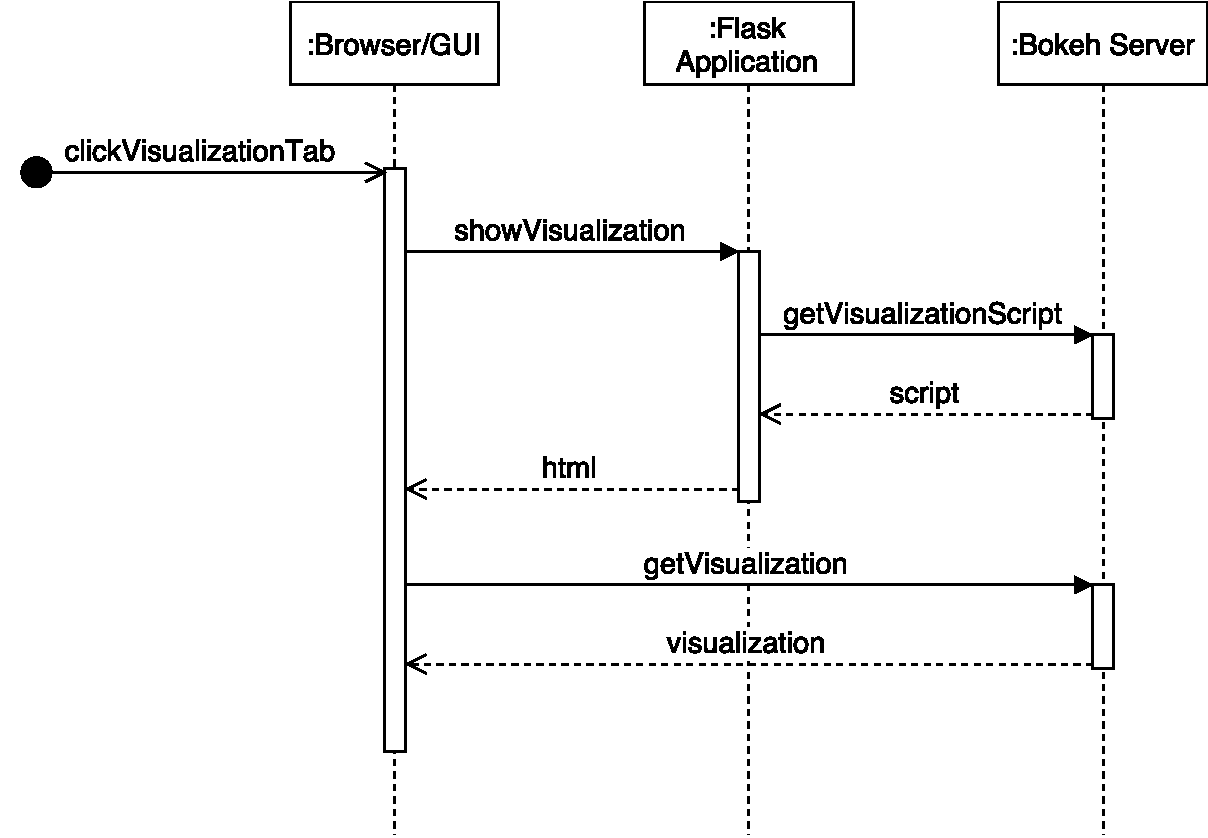
\includegraphics[width=\textwidth]{fig/sequence-bokeh.pdf}
        \caption{Sequence diagram of getting a visualization from Bokeh Server}
        \label{fig:bokeh-server}
\end{figure}

\subsection{Bokeh Applications}

As mentioned, a Bokeh application is created for each visualization technique, resulting in the following five applications:

\begin{itemize}
    \item \texttt{deconvolutional\_network.py}
    \item \texttt{deep\_visualization.py}
    \item \texttt{layer\_activations.py}
    \item \texttt{saliency\_maps.py}
    \item \texttt{training\_progress.py}
\end{itemize}

\noindent We will not describe the implementation of the applications in detail. Most parts of the code deals with the creation and updating of figures using functions provided by Bokeh, which is not particularly interesting for the thesis. Rather, we will present some of the most important concepts of the implementations. The resulting visualization can be seen in \autoref{chap:results}.

\subsubsection{Handling the Visualization Data}

All of the Bokeh applications begin with the same lines of code, shown in \autoref{code:visualization-files}. The document variable in line 1 holds the current Bokeh document that we are working on. In lines 2-5, we get the HTTP request arguments from the Flask request. These arguments are used to find the path in the user storage corresponding to the file we are going to visualize data for, as seen in line 7. \texttt{UPLOAD\_FOLDER} is the path to the user storage folder, imported from the configuration file. Some of the Bokeh applications also display the original image used in the visualization. This image is found using a similar method as for the visualization files. \\

\begin{listing}[h!]
\begin{minted}
[
frame=lines,
framesep=2mm,
baselinestretch=1.2,
fontsize=\footnotesize,
linenos
]
{python}
document = curdoc()
args = document.session_context.request.arguments

file = args['file'][0].decode('ascii')
user = args['user'][0].decode('ascii')

results_path = join(UPLOAD_FOLDER, user, file, 'results')
\end{minted}
\caption{Getting the data from the visualization files}
\label{code:visualization-files}
\end{listing}

\noindent The data loaded from the visualization file is processed to a format that is beneficial for presentation. The processing depends on the specific visualization technique, and the format of the visualization files can be seen in \autoref{app:visualization-files}. For instance, data for the training progress is transformed from rows of x- and y-values into separate sequences of x- and y-values. The other techniques mostly output image data, which needs to be converted into 2D arrays, since Bokeh does not handle 3D arrays for images. For layer activations, the results include a large amount of images for the convolutional layers. These are stitched together into a grid of images for each layer. When the data has been properly processed, it is stored in a \texttt{ColumnDataSource}, a Bokeh object that stores data to be used in a figure. In our case, its main purpose is to allow for simple streaming of data. When associating a ColumnDataSource with a figure, updating the data of the \texttt{ColumnDataSource} automatically triggers an update of the figure. This approach is much more efficient than creating a new figure every time the data is updated. The update is performed by adding a periodic Bokeh callback to a function that reads the visualization file and updates the data of the \texttt{ColumnDataSource}. The interval of this update is defined by the Flask configuration file.

\section{Case Study in Face Recognition}

In this section, we describe the implementation details concerning the case study. To begin with, we explain how expression information can be useful, and then present ideas about how experimental networks can utilize this information. Subsequently, we provide insight into our methods for obtaining satisfactory networks based on these ideas. We then examine a pretrained model, which was used as a feature extractor for the case study networks. Next we introduce the dataset used to investigate our theory, and how the images of this set were preprocessed. Finally, nine different architectures are suggested, three for each network variation. These architectures are considered to be separate from the pretrained network, but using its feature output as input. Note that these architectures are all specified using the Keras 2 \acrshort{api} terminology.

\subsection{Exploiting Expression Information}

The way facial expressions alter the facial geometry is predictable, both in a specific and general sense. If a specific person conveys the same facial expression several times, the expression will consistently affect a certain set of features and always in a similar manner. For instance, if an image of a happy person includes feature variations such as a widened mouth, narrower eyes, and dimples, another image of that person being happy will likely include the same variations. Some alterations can also be expected to appear generally. While dimples are not a universal trait, a smile, causing a wider mouth, can be anticipated to be commonplace in facial expressions conveying happiness. Knowing or recognizing the facial expression of a person would then reveal some information about how the facial features have transformed in relation to the person's neutral features. This case study examines how to exploit this predictability by including facial expression data in the \acrshort{ann} training procedure. If a face recognition system could learn how these expressions affect facial geometry, then the system could be able to match the dissimilarities in the facial features with the changes it knows the facial expression produces. This way, we can move away from trying to overcome the expression challenge through invariance, and instead utilize the data about facial expressions to increase network performance.

\subsection{Experimental Network Idea}

For the case study, we wanted to examine if the performance of a face recognition network could be improved by incorporating facial expression data. To examine this idea, we considered three different neural network approaches for facial recognition. The first network was used as a standard to be measured up against, with no utilization of expression data. It simply receives an input image and emits an identity classification result as output, determining who the individual in the image is. The second network receives the facial expression of the person in the image as input, in addition to the input image. The output will be similar to the standard network. This network has the potential to use the expression data explicitly, to learn how the expressions alter which facial features match the various identities. The third network outputs both the identification classification result and a facial expression classification for the input image person, without receiving any extra input. By trying to classify both identification and expression simultaneously, the network has the potential to learn how the facial features and expressions relate to each other. The network would then implicitly learn how the expression input alters the facial features, which could improve identification classification. The performance of each network is measured by its total classification loss and accuracy. To simplify the training of these networks, a pretrained network was used as a feature extractor. A large, shared part of the networks is then already fully trained, leaving only the classification part, greatly decreasing the time required for training. Reducing the training time allows for more extensive experimentation. 

\subsection{Method}

When creating the case study networks, we started by identifying advantageous baseline structures. To examine the performance, we used the tool described in this thesis to visualize the training progress, monitoring loss and accuracy for the training and validation sets. For the architectures with an extra output, these metrics were read manually from a log file, as the tool does not support training progress visualization for networks with multiple outputs. The other visualization techniques were not utilized due to the incompatibility with non-sequential networks, the homogeneity of the dataset, and the classification importance of relatively fine details. \\

\noindent The architectures that were investigated varied in depth and width, i.e. in the amount of units per layer. In addition, we explored different levels of regularization strength, which was determined both by how many layers experienced dropout and how high the rate of dropout was for each layer. We also looked into how different training hyperparameters affected the network, observing how they learned using various epochs and batch sizes, as well as different adaptive learning algorithms and initial learning rates. \\

\noindent After establishing a selection of satisfactory baseline architectures, we used them as starting points for the creation of the experimental networks. If any of the adaptions showed promise, we explored them further by adjusting depth and width, and experimenting with training length and the initial learning rate. For every new architecture, we kept any that offered improvements, quickly discarding those that failed to enhance performance, because of the large amount of potential configurations. Specific to the architectures utilizing an extra input, we investigated how the networks reacted to injecting the input at various locations. For the architectures that were required to output an extra classification result, we varied the amount of layers that were connected to both output layers and the amount of layers that were only connected to one of them. If we discovered an experimental network that performed admirably, but lacked a baseline counterpart, we also tested the corresponding baseline architecture. Through these incremental improvements, we discovered the final architectures described in \autoref{sec:case-networks}. 

\subsection{Pretrained Model}

As described in \autoref{sec:transfer-learning}, transfer learning is an appropriate method for training an \acrshort{ann} without extensive training time or large amounts of training data. To employ transfer learning, a suitable pretrained model is needed. Since our case study deals with face recognition, it would be beneficial to use a \acrshort{cnn} that was previously trained for such a purpose. The network would then already be able to detect specific facial features, like mouths and eyes. A suitable model is the 16 weight layer D configuration of the \acrshort{vgg}-Face \acrshort{cnn} \cite{deep-face-rec}. The weight values of this configuration, as computed in Parki et al. \cite{deep-face-rec}, has been made available\footnote{http://www.robots.ox.ac.uk/~vgg/software/vgg\_face/} and converted to use with the Keras framework\footnote{https://github.com/rcmalli/keras-vggface}. This particular configuration will be referred to as the \acrshort{vgg}-Face network from here on out. The original implementation used Caffe\footnote{http://caffe.berkeleyvision.org/}, but we will be using a Keras implementation converted from the original Caffe network. The Keras version allows us to utilize the visualization tool for managing the various networks created and visualizing certain data. We describe the architecture here, with the full implementation found at GitHub\footnote{https://github.com/rcmalli/keras-vggface}. \\

\noindent An overview of the pretrained network architecture is shown in \autoref{tab:vggface-arch}. Here, the network has 25 layers, including the input layer. However, only 15 of the layers have weights associated with them. If we add the excluded classification output layer, the number rises to 16. This architecture is based on the network that is popularly called \acrshort{vgg}-16 \cite{vgg}, which was originally applied to \acrshort{ilsvrc} \cite{imagenet}. The architecture as demonstrated praiseworthy performance in face recognition and \acrshort{ilsvrc} object classification, which both require excellent feature extraction capabilities. The feature extraction proficiency is made possible by the stacked convolutional layers, with max pooling layers to obtain some spatial invariance. All the convolutional filters are of size 3x3, which for the first layer is enough to capture small, simple features. The complexity of the features grows with the depth of the layers, each layer capturing features made up of lower level features. Depth also increases the effective receptive fields of the layer units, as they become indirectly connected to a larger number of input units. The fully connected layers are indirectly connected to every input unit, and are used to combine the extracted features of the convolutional layers to create even more complex and invariant feature representations. \\


\begin{table}[h!]
\begin{center}
\begin{tabular}{|c|c|c|c|}
\hline
\textbf{Layer \#} & \textbf{Name} & \textbf{Layer Type} & \textbf{Units} \\ \hline
0 & input & InputLayer & 224x224x3  \\ \hline
1 & conv1\_1 & \multirow{2}{*}{Conv2D} & \multirow{2}{*}{224x224x64} \\ \cline{1-2}
2 & conv1\_2 & & \\ \hline
3 & pool1 & MaxPooling2D & 112x112x64 \\ \hline
4 & conv2\_1 & \multirow{2}{*}{Conv2D} & \multirow{2}{*}{112x112x128} \\ \cline{1-2}
5 & conv2\_2 & & \\ \hline
6 & pool2 & MaxPooling2D & 56x56x128 \\ \hline
7 & conv3\_1 & \multirow{3}{*}{Conv2D} & \multirow{3}{*}{56x56x256} \\ \cline{1-2}
8 & conv3\_2 & & \\ \cline{1-2}
10 & conv3\_3 & & \\ \hline
11 & pool3 & MaxPooling2D & 23x23x256 \\ \hline
12 & conv4\_1 & \multirow{3}{*}{Conv2D} & \multirow{3}{*}{23x23x512} \\ \cline{1-2}
13 & conv4\_2 & & \\ \cline{1-2}
14 & conv4\_3 & & \\ \hline
15 & pool4 & MaxPooling2D & 11x11x512 \\ \hline
16 & conv4\_1 & \multirow{3}{*}{Conv2D} & \multirow{3}{*}{11x11x512} \\ \cline{1-2}
17 & conv4\_2 & & \\ \cline{1-2}
18 & conv4\_3 & & \\ \hline
19 & pool5 & MaxPooling2D & 5x5x512 \\ \hline
20 & flatten & Flatten & 12800 \\ \hline
21 & fc6 & Dense & \multirow{4}{*}{4096} \\ \cline{1-3}
22 & fc6/relu & Activation & \\ \cline{1-3}
23 & fc7 & Dense & \\ \cline{1-3}
24 & fc7/relu & Activation & \\ \hline
\end{tabular}
\end{center}
\caption[Pretrained network architecture]{Pretrained network architecture. The last two layers of the original model have been excluded, as these form the classification output and are therefore irrelevant. Note that the layer type refers to the Keras 2 \acrshort{api}. All Conv2D layers use 3x3 filters, with single strides, same convolution padding, and \acrshort{relu} activation functions. All MaxPooling2D layers use 2x2 pooling regions, with double strides and no padding. Flatten layer simply flattens input. Both Dense (fully connected) layers have linear activation functions, but are followed by an Activation layer using \acrshort{relu} activation functions.}
\label{tab:vggface-arch}
\end{table}

\subsection{Dataset and Preprocessing}

Based on the restrictions regarding the dataset described in \autoref{sec:data-generation-methods}, as well as the review of potential datasets conducted in the Specialization Project, the \acrfull{imfdb} \cite{imfdb} was selected to be used in the case study. The database consists of 34,512 images of 100 actors collected from Indian movies, captured in an unconstrained setting. All images have been selected and labeled manually, and the labels include both identification and expression. The available expressions are the six basic expressions described in \autoref{sec:facial-expressions}, in addition to a neutral expression, giving a total of seven possible values for the expression label. The dataset is structured so that it contains a folder for each of the actors. These folders again contain a folder for every movie where actor images were extracted. A movie folder contain an image folder and a text file with all image names and their corresponding labels. \\

\noindent After downloading the dataset, we received some errors while trying to process the text files. Thus, we created a script that traversed the text files of the dataset and alerted us of any peculiarities. Some of the entries were missing their expression labeling and these were removed entirely. Others were just improperly formatted, which was easily fixed. This process reduced the number of images, resulting in a dataset with 30,091 images of 98 actors. The dataset was then split into three sets consisting of 70\%, 20\% and 10\% of the images. These sets were used for training, validation and testing, respectively. The images were already cropped with a tight bounding box around the faces, thus the only preprocesssing needed to use the images with the \acrshort{vgg}-Face network were scaling and padding. The images were padded to squares with black, and scaled to an appropriate size of 130x130 pixels. The size was selected on the background of the mean image width and height of the dataset, which was calculated to be 102 and 129, respectively. \\

\noindent Although \acrshort{imfdb} provides everything we need in terms of labels, the quality of the dataset is debatable. When processing the dataset, we discovered that the smallest image is only 8x11 pixels in size. In comparison, the largest image is 852x893 pixels. Some of the images are small and of poor quality, but since having a large amount of images was a crucial factor to our case, we decided to keep all of them hoping that the general overall quality would be good enough. Another issue is the reliability of the expression labeling. As the images are captured in an unconstrained setting, it may be problematic to assign appropriate expressions to every image. There are many ways to express an emotion, and the classification of an emotion based on a person's facial expression is a subjective process. A random selection of images from the dataset, labeled with each of the seven expression values, can be seen in \autoref{fig:imfdb-images}. It is evident that some of the labels seem more obvious and fitting than others. However, datasets captured in constrained settings were found to contain a significantly smaller number of images, as they all need to be captured manually. Unconstrained images are more easily retrieved in large amounts exploiting existing images on the Internet or still images from movies. Another advantage with employing an unconstrained dataset like \acrshort{imfdb} is that the pretrained model was trained on such images, and it is convenient to utilize a similar dataset when conducting transfer learning.

\begin{figure}
\captionsetup[subfigure]{labelformat=empty}
\begin{center}
\begin{tabular}{ccccccc}
\subfloat[Neutral]{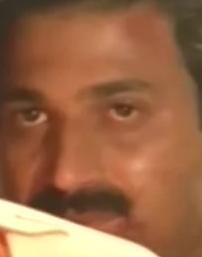
\includegraphics[width = 0.5in]{fig/IMFDB/Siddique_234_neutral.jpg}} &
\subfloat[Happiness]{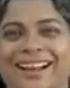
\includegraphics[width = 0.5in]{fig/IMFDB/Umashri_5_happiness.jpg}} &
\subfloat[Surprise]{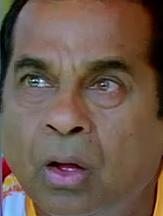
\includegraphics[width = 0.5in]{fig/IMFDB/Brahmanadam_109_surprise.jpg}} &
\subfloat[Sadness]{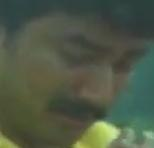
\includegraphics[width = 0.5in]{fig/IMFDB/Jayaram_22_sadness.jpg}} &
\subfloat[Anger]{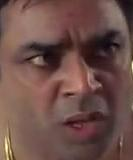
\includegraphics[width = 0.5in]{fig/IMFDB/PareshRaval_57_anger.jpg}} & 
\subfloat[Disgust]{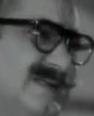
\includegraphics[width = 0.5in]{fig/IMFDB/SVR_133_disgust.jpg}} &
\subfloat[Fear]{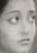
\includegraphics[width = 0.5in]{fig/IMFDB/Jamuna_11_fear.jpg}} \\
\end{tabular}
\caption[Images from \acrshort{imfdb}]{A labeled selection of images from \acrshort{imfdb}, one for each expression.}
\label{fig:imfdb-images}
\end{center}
\end{figure}

\subsection{Case Study Networks} \label{sec:case-networks}

All of the case study networks use the pretrained network as a fixed base. Hence, they can be viewed as separate networks whose input is shaped similarly to the pretrained network's output. We therefore describe the different architectures for the case study networks with no explicit connection to the pretrained network and consider the input to be a feature vector of size 4096. Should any of the architectures defined here be applied to images, they would need to be combined with the pretrained model. For each of the three approaches, we have included three architectures. For every approach, the three architectures consist of a minimal architecture, the architecture with the best performance, and an interesting alternative to the preferred architecture. The minimal and alternate architectures are included as comparisons to the preferred one, to help determine what makes the preferred architecture excel. \\

\noindent It is worth noticing that every selected architecture has a dropout layer right after the input layer. This was added as a standard because of the most basic baseline, where only an output layer was added, which quickly achieved 100\% training accuracy and a very low loss value. The validation accuracy and loss, however, were stuck at less beneficial values. Naturally, overfitting was suspected, and while it became apparent in the later stages of training, the main issue was the lack of progress. By utilizing dropout on the feature input, the network had a harder time fitting perfectly to the data, and it showed a slight improvement in the validation metrics. Generally, the architectures are heavily regularized with dropout due to overfitting concerns, as it had a tendency to arise in architectures with less utilization of the dropout technique. The tendency to overfit is most likely caused by the relatively small size of the dataset used. In turn, this tendency restricted architecture exploration, as deeper architectures systematically overfitted and had unsatisfactory performance. \\

\subsubsection{Baseline Configurations}

The three baseline architecture configurations A, B and C are shown in \autoref{tab:base-arch}. A is the minimal architecture, with only a dropout layer between the input and output layers. B is the preferred baseline architecture. It includes a couple of fully connected layers, each followed by a dropout layer. This extra depth offers an improvement over the minimal approach, suggesting that the model benefits from a more complex classifier. The alternative architecture, C, is one fully connected and one dropout layer deeper than B. Although having the potential of an even more complex classifier, this architecture performed worse than B. Most likely, it is caused by overfitting as a result of the increased number of parameters. However, the performance remains stable, even after many epochs, implying that the network was somewhat overfitted before it was able to achieve a loss and accuracy on par with configuration B.

\begin{table}[h!]
\begin{center}
\begin{tabular}{|c|c|c|c|c|}
\hline
\textbf{Config.} & \textbf{Layer \#} & \textbf{Name} & \textbf{Layer Type} & \textbf{Units} \\ \hline
\multirow{3}{*}{A} & 0 & input & InputLayer & \multirow{2}{*}{4096} \\ \cline{2-4}
 & 1 & drop & Dropout & \\ \cline{2-5}
 & 2 & output & Dense & 98 \\ \hline
\multirow{7}{*}{B} & 0 & input & InputLayer & \multirow{2}{*}{4096} \\ \cline{2-4}
 & 1 & drop1 & Dropout & \\ \cline{2-5}
 & 2 & fc1 & Dense & \multirow{4}{*}{1024} \\ \cline{2-4}
 & 3 & drop2 & Dropout & \\ \cline{2-4}
 & 4 & fc2 & Dense & \\ \cline{2-4}
 & 5 & drop3 & Dropout & \\ \cline{2-5}
 & 6 & output & Dense & 98 \\ \hline
\multirow{9}{*}{C} & 0 & input & InputLayer & \multirow{2}{*}{4096} \\ \cline{2-4}
 & 1 & drop1 & Dropout & \\ \cline{2-5}
 & 2 & fc1 & Dense & \multirow{6}{*}{1024} \\ \cline{2-4}
 & 3 & drop2 & Dropout & \\ \cline{2-4}
 & 4 & fc2 & Dense & \\ \cline{2-4}
 & 5 & drop3 & Dropout & \\ \cline{2-4}
 & 6 & fc3 & Dense & \\ \cline{2-4}
 & 7 & drop4 & Dropout & \\ \cline{2-5}
 & 8 & output & Dense & 98 \\ \hline
\end{tabular}
\end{center}
\caption[Baseline architecture configurations]{Baseline network architecture configurations. Note that the layer type refers to the Keras 2 \acrshort{api}. All Dense (fully connected) layers use \acrshort{relu} activation functions, except the output layer of every configuration, which use softmax. All Dropout layers use a 0.5 dropout rate.}
\label{tab:base-arch}
\end{table}

\subsubsection{Extra Input Configurations}

The three architectures with an additional expression input, with configurations D, E and F, are shown in \autoref{tab:ex-in-arch}. These architectures have multiple inputs and therefore the layers do not follow a fully sequential order. Rather, they each have two branches which merge together at some point. The layer numbering X-Y suggests this, where X denotes the consecutive order and Y denotes the branch it belongs to. The branches are merged in the concatenate layer by concatenating the output of the preceding layer branches. For every configuration, the concatenate layer is where the expression input is incorporated, without any layers in between. The feature input layer, however, has a varying degree layers between it and the concatenate layer, allowing the network to do some computation on the feature input alone before employing the expression data. \\

\noindent Of these configurations, D is the minimal, E is the preferred, and F is the alternate. Compared to the baseline configurations, D is similar to A, while E and F are similar to B. In D, the extra input is added right after the dropout layer. Networks with this architecture can then only use a single layer, the output, to make sense of the combined inputs. E allows a little more leeway, with an additional fully connected and dropout layer pair both before and after the facial expression input is injected. Its only difference to the baseline configuration B, is the additional input. The first fully connected layer allows for some processing of the feature input alone, before its output is processed in combination with the expression input in the following fully connected layers, the last of them outputting an identification classification. As with B, however, deepening the network produced no further improvement, with networks not achieving similar performance and rather showing signs of overfitting. Lastly, F inserts the expression input right after the initial dropout layer. A network with this configuration does perform better than D, but never reaches the performance levels of E, supporting the benefit of additional processing of the feature input. 

\begin{table}[h!]
\begin{center}
\begin{tabular}{|c|c|c|c|c|}
\hline
\textbf{Config.} & \textbf{Layer \#} & \textbf{Name} & \textbf{Layer Type} & \textbf{Units} \\ \hline
\multirow{5}{*}{D} & 0-1 & exp\_input & \multirow{2}{*}{InputLayer} & 7 \\ \cline{2-3} \cline{5-5}
 & 0-2 & feat\_input & & \multirow{2}{*}{4096} \\ \cline{2-4}
 & 1-2 & drop & Dropout & \\ \cline{2-5}
 & 2 & concat & Concatenate & 4103 \\ \cline{2-5}
 & 3 & output & Dense & 98 \\ \hline
\multirow{9}{*}{E} & 0-0 & exp\_input & \multirow{2}{*}{InputLayer} & 7 \\ \cline{2-3} \cline{5-5}
 & 0-2 & feat\_input & & \multirow{2}{*}{4096} \\ \cline{2-4}
 & 1-2 & drop1 & Dropout & \\ \cline{2-5}
 & 2-2 & fc1 & Dense & \multirow{2}{*}{1024} \\ \cline{2-4}
 & 3-2 & drop2 & Dropout & \\ \cline{2-5}
 & 4 & concat & Concatenate & 1031 \\ \cline{2-5}
 & 5 & fc2 & Dense & \multirow{2}{*}{1024} \\ \cline{2-4}
 & 6 & drop3 & Dropout & \\ \cline{2-5}
 & 7 & output & Dense & 98 \\ \hline
\multirow{9}{*}{F} & 0-1 & exp\_input & \multirow{2}{*}{InputLayer} & 7 \\ \cline{2-3} \cline{5-5}
 & 0-2 & feat\_input & & \multirow{2}{*}{4096} \\ \cline{2-4}
 & 1-2 & drop1 & Dropout & \\ \cline{2-5}
 & 2 & concat & Concatenate & 4103 \\ \cline{2-5}
 & 3 & fc1 & Dense & \multirow{4}{*}{1024} \\ \cline{2-4}
 & 4 & drop2 & Dropout & \\ \cline{2-4}
 & 5 & fc2 & Dense & \\ \cline{2-4}
 & 6 & drop3 & Dropout & \\ \cline{2-5}
 & 7 & output & Dense & 98 \\ \hline 
\end{tabular}
\end{center}
\caption[Extra input architecture configurations]{Extra input network architecture configurations. Note that the layer type refers to the Keras 2 \acrshort{api}. Architectures are not fully sequential, with some layers only appearing in certain branches. Layers in branches have X-Y layer numbers, with X referring to layer number and Y referring to branch number. All Dense (fully connected) layers use \acrshort{relu} activation functions, except the output layer of every configuration, which use softmax. All Dropout layers use a 0.5 dropout rate. The Concatenate layer is used to merge branches, by concatenating the output from the branches in the preceding layers.}
\label{tab:ex-in-arch}
\end{table}


\subsubsection{Extra Output Configurations}

The architecture configurations having an extra expression output are named G, H and I, and are shown in \autoref{tab:ex-out-arch}. Similar to the extra input architectures, these architectures have branches, and the layer numbering scheme for branches is identical. Unlike the extra input case, however, G, H and I never merge the branches. A network of this architecture would then output two separate results, one for identification and one for expression. As a result, the model would also have multiple loss and accuracy values, one for each output layer. Consequently, the visualization tool cannot be used for these networks, as it does not support multiple values for each metric. Although it is the face recognition part of the network we are truly interested in, it is unlikely that a network would gain an identification classification advantage from the enforced simultaneous classification if the expression results are underwhelming. To examine the extra output configurations, we must therefore consider the performance results for both classification tasks. The extra output networks are then supposed to do more than both the previous approaches, with no additional information. \\

\noindent In test architectures that tried to classify only the facial expression, validation accuracy did not rise far above 50\%, suggesting that the networks had difficulty using the feature input to classify expressions. This may very well be a result of the chosen pretrained model, which was trained to recognize faces and thus has learned to prioritize features which help with identification, not expression classification. It seems that there might be some overlap between the features used to classify identification and expression, but not enough to use the pretrained model as a feature extractor in a proper expression classifier. Naturally, this lack of focus on important expression features inhibits the extra output architectures, which are tasked with classifying both the identification and expression. \\

\noindent G is the minimal approach, H is the preferred and I is the alternate. G resembles baseline configuration A, with the distinction that the dropout layer forwards its values to two output layers instead of one. In this configuration, the input to the identification output layer and the expression output layer is not processed by any common layers that employ weights. H shares similarities with B, having two fully connected layers, separated by dropout layers, before the identification output layer. An additional fully connected layer, followed by dropout, is employed prior to the expression output layer. The two first fully connected layers are shared by the output layers and are influenced by both during training, while the \texttt{fc3} layer is only affected by the backpropagation updates from the expression output layer. We can consider the computations of the layers that are only affected by one output layer as specialized processing for the specific classification task. The final configuration, I, is similar to H, but has identification specific processing instead of expression specific processing. The change leads to poorer overall performance compared to H, and, interestingly, the identification performance of I can be improved by removing the specialized layer. The situation is likely similar to the baseline configuration C, where the additional parameters enable overfitting. Doing the equivalent to H, on the other hand, would result in an expression performance decrease. This demonstrates the need for further and more specialized processing of the features to gain a satisfactory expression classification. This is somewhat unsurprising, regarding the lack of focus on expressions in the pretrained model, as previously mentioned. A network with specialized processing for both classifications has identification and expression performance similar to I and H, respectively. This aligns with the previous observations that specific identification processing causes harm, while specific expression processing is beneficial.

\begin{table}[h!]
\begin{center}
\begin{tabular}{|c|c|c|c|c|}
\hline
\textbf{Config.} & \textbf{Layer \#} & \textbf{Name} & \textbf{Layer Type} & \textbf{Units} \\ \hline
\multirow{4}{*}{G} & 0 & input & InputLayer & \multirow{2}{*}{4096} \\ \cline{2-4}
& 1 & drop & Dropout & \\ \cline{2-5}
& 2-1 & id\_output & \multirow{2}{*}{Dense} & 98 \\ \cline{2-3} \cline{5-5}
& 2-2 & exp\_output & & 7 \\ \hline
\multirow{10}{*}{H} & 0 & input & InputLayer & \multirow{2}{*}{4096} \\ \cline{2-4}
& 1 & drop1 & Dropout & \\ \cline{2-5}
& 2 & fc1 & Dense & \multirow{4}{*}{1024} \\ \cline{2-4}
& 3 & drop2 & Dropout & \\ \cline{2-4}
& 4 & fc2 & Dense & \\ \cline{2-4}
& 5 & drop3 & Dropout & \\ \cline{2-5}
& 6-1 & id\_output & \multirow{2}{*}{Dense} & 98 \\ \cline{2-3} \cline{5-5}
& 6-2 & fc3 & & \multirow{2}{*}{1024} \\ \cline{2-4}
& 7-2 & drop4 & Dropout & \\ \cline{2-5}
& 8-2 & exp\_output & Dense & 7 \\ \hline
\multirow{10}{*}{I} & 0 & input & InputLayer & \multirow{2}{*}{4096} \\ \cline{2-4}
& 1 & drop1 & Dropout & \\ \cline{2-5}
& 2 & fc1 & Dense & \multirow{4}{*}{1024} \\ \cline{2-4}
& 3 & drop2 & Dropout & \\ \cline{2-4}
& 4 & fc2 & Dense & \\ \cline{2-4}
& 5 & drop3 & Dropout & \\ \cline{2-5}
& 6-1 & exp\_output & \multirow{2}{*}{Dense} & 7 \\ \cline{2-3} \cline{5-5}
& 6-2 & fc3 & & \multirow{2}{*}{1024} \\ \cline{2-4}
& 7-2 & drop4 & Dropout & \\ \cline{2-5}
& 8-2 & id\_output & Dense & 98 \\ \hline
\end{tabular}
\end{center}
\caption[Extra output architecture configurations]{Extra output network architecture configurations. Note that the layer type refers to the Keras 2 \acrshort{api}. Architectures are not fully sequential, with some layers only appearing in certain branches. Layers in branches have X-Y layer numbers, with X referring to layer number and Y referring to branch number. All Dense (fully connected) layers use \acrshort{relu} activation functions, except the output layers of every configuration, which use softmax. All Dropout layers use a 0.5 dropout rate. The output of each configuration comes from the two output layers.}
\label{tab:ex-out-arch}
\end{table}


\cleardoublepage